\documentclass{article}

\usepackage{booktabs}
\usepackage{graphicx}
\usepackage{caption}
\usepackage{subcaption}

\title{Searching for Pump and Dump: Initial Analysis}
\author{Ivan Anich}

\graphicspath{{../dev/}}

\begin{document}
\maketitle

This is an initial analysis of a pond I'm calling `Pump and Dump'. I have not yet been able to identify a pump and dump signal, but the results below are very promising, regardless.

\section{The Signal}

The default signal analyzed is a rise of at least 20\% from the open and a close less than \$2 but at least \$1. Over trading days between December 29th, 2020 and May 20th 2021, this signal was observed 408 times among 186 unique tickers. There is some seasonality in the frequency of this signal: before February 26th, 2021 the signal was observed 286 times, after that date it was observed 122 times. Performance has been much better after this date, and I have provided an additional analyses of performance in this timeframe.

I also analyze a variant of the default in which only stocks that rise 32\% are entered. 32\% is the average rise of the stocks in who show the default signal.

One warning about this signal. The `close between \$2 and \$1' could pose a problem. If you are entering trades on the day that the stock rises 20\%, you are doing so before observing whether the stock closes between \$1 and \$2. I assume that you will look for stocks that rise 20\% that are currently priced between \$1 and \$2. If these stocks perform systematically differently from stocks that \textit{close} between \$1 and \$2 perform, the below results will be as inaccurate as those systematic differences.

\section{Results: Default Signal, Entry at 20\%}

The first scenario I analyzed was a short sale with an entry at the 20\% above open level. By construction, all observations met this criteria. Table \ref{tab_var_1} summarizes the analysis, grouping results by winners and losers, and figure \ref{fig_var_1_ext_hold} shows a break down of returns for holding positions beyond the entry day. A day 0 exit is the optimal exit day.

For an exit on the same day of entry, the win rate was 66\%, with a 8.5:11 win-loss ratio, and an expected return of 2\%. 

\begin{table}
\caption{Performance of Default Signal, Entry at 20\%}
\center{Winners}
\\[2ex]
\begin{tabular}{lcccc}
\hline
         &   0.25   &   0.75   &  median  & average   \\
\midrule
\midrule
constant & 0.0337   & 0.1087   & 0.0676   & 0.0851    \\
         & (0.0033) & (0.0064) & (0.0043) & (0.0046)  \\
N        & 271      & 271      & 271      & 271       \\
Win rate & 0.66     & 0.66     & 0.66     & 0.66      \\
\hline
\end{tabular}

\center{Losers}
\\[2ex]
\begin{tabular}{lcccc}
\hline
          &   0.25   &   0.75   &  median  & average   \\
\midrule
\midrule
constant  & 0.0177   & 0.1297   & 0.0476   & 0.1092    \\
          & (0.0063) & (0.0193) & (0.0075) & (0.0194)  \\
N         & 134      & 134      & 134      & 134       \\
Loss rate & 0.33     & 0.33     & 0.33     & 0.33      \\
\hline
\end{tabular}
\label{tab_var_1}
\end{table}

\begin{figure}
\center{Default Signal, 20\% Entry: Average and Quantile Returns By Day Held}
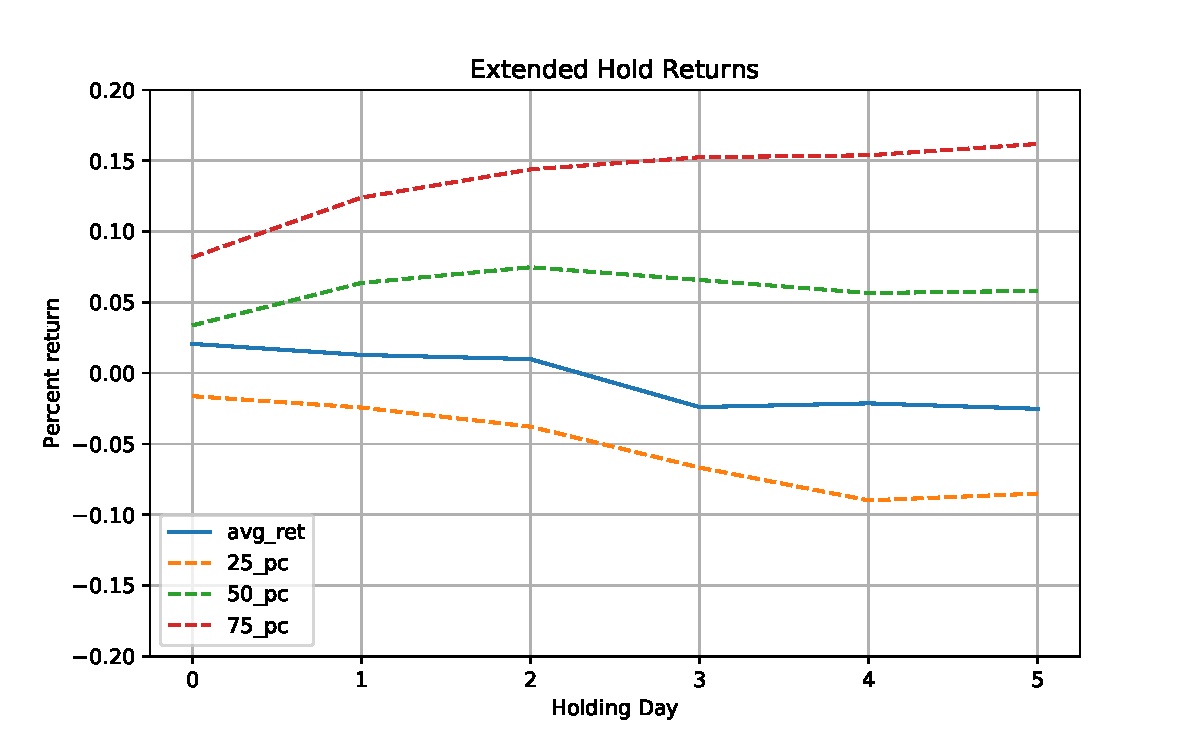
\includegraphics[width=\textwidth]{pump_dump_ext_hold_var_1.pdf}
\caption{Extended hold returns are shown. Returns on a holding day are the return if the position was exited on the holding day in question. For example, returns on holding day 0 are returns in stocks were sold at the day the position was entered; returns on day 1, for stocks sold after holding for one day. The quantile returns represent the fraction of stocks with returns worse than the dashed line. for example, the red dashed line shows that 75\% of stocks had returns worse than ~8\% on day 0, ~12.5\% on day 1, etc.}
\label{fig_var_1_ext_hold}
\end{figure}

I simulated a trading strategy in which 10\% of a \$25,000 portfolio is exposed to the signal. Exposure compounds, and is evenly spread each day among any and all stocks that meet the aforementioned signal: entry occurs at 20\% above open. Figure \ref{fig_var_1_sim} shows the results of the simulation. One striking feature of figure \label{fig_var_1_sim} is the drop off in the number of trades each day around day 40 of the simulation. This is around February 26th, the aforementioned date at which it appears the market changed. Before this date, the number of trades per day is so high as to make execution of the strategy far more difficult.

\begin{figure}
\caption{Default Signal, 20\% Entry: Simulation}
\center
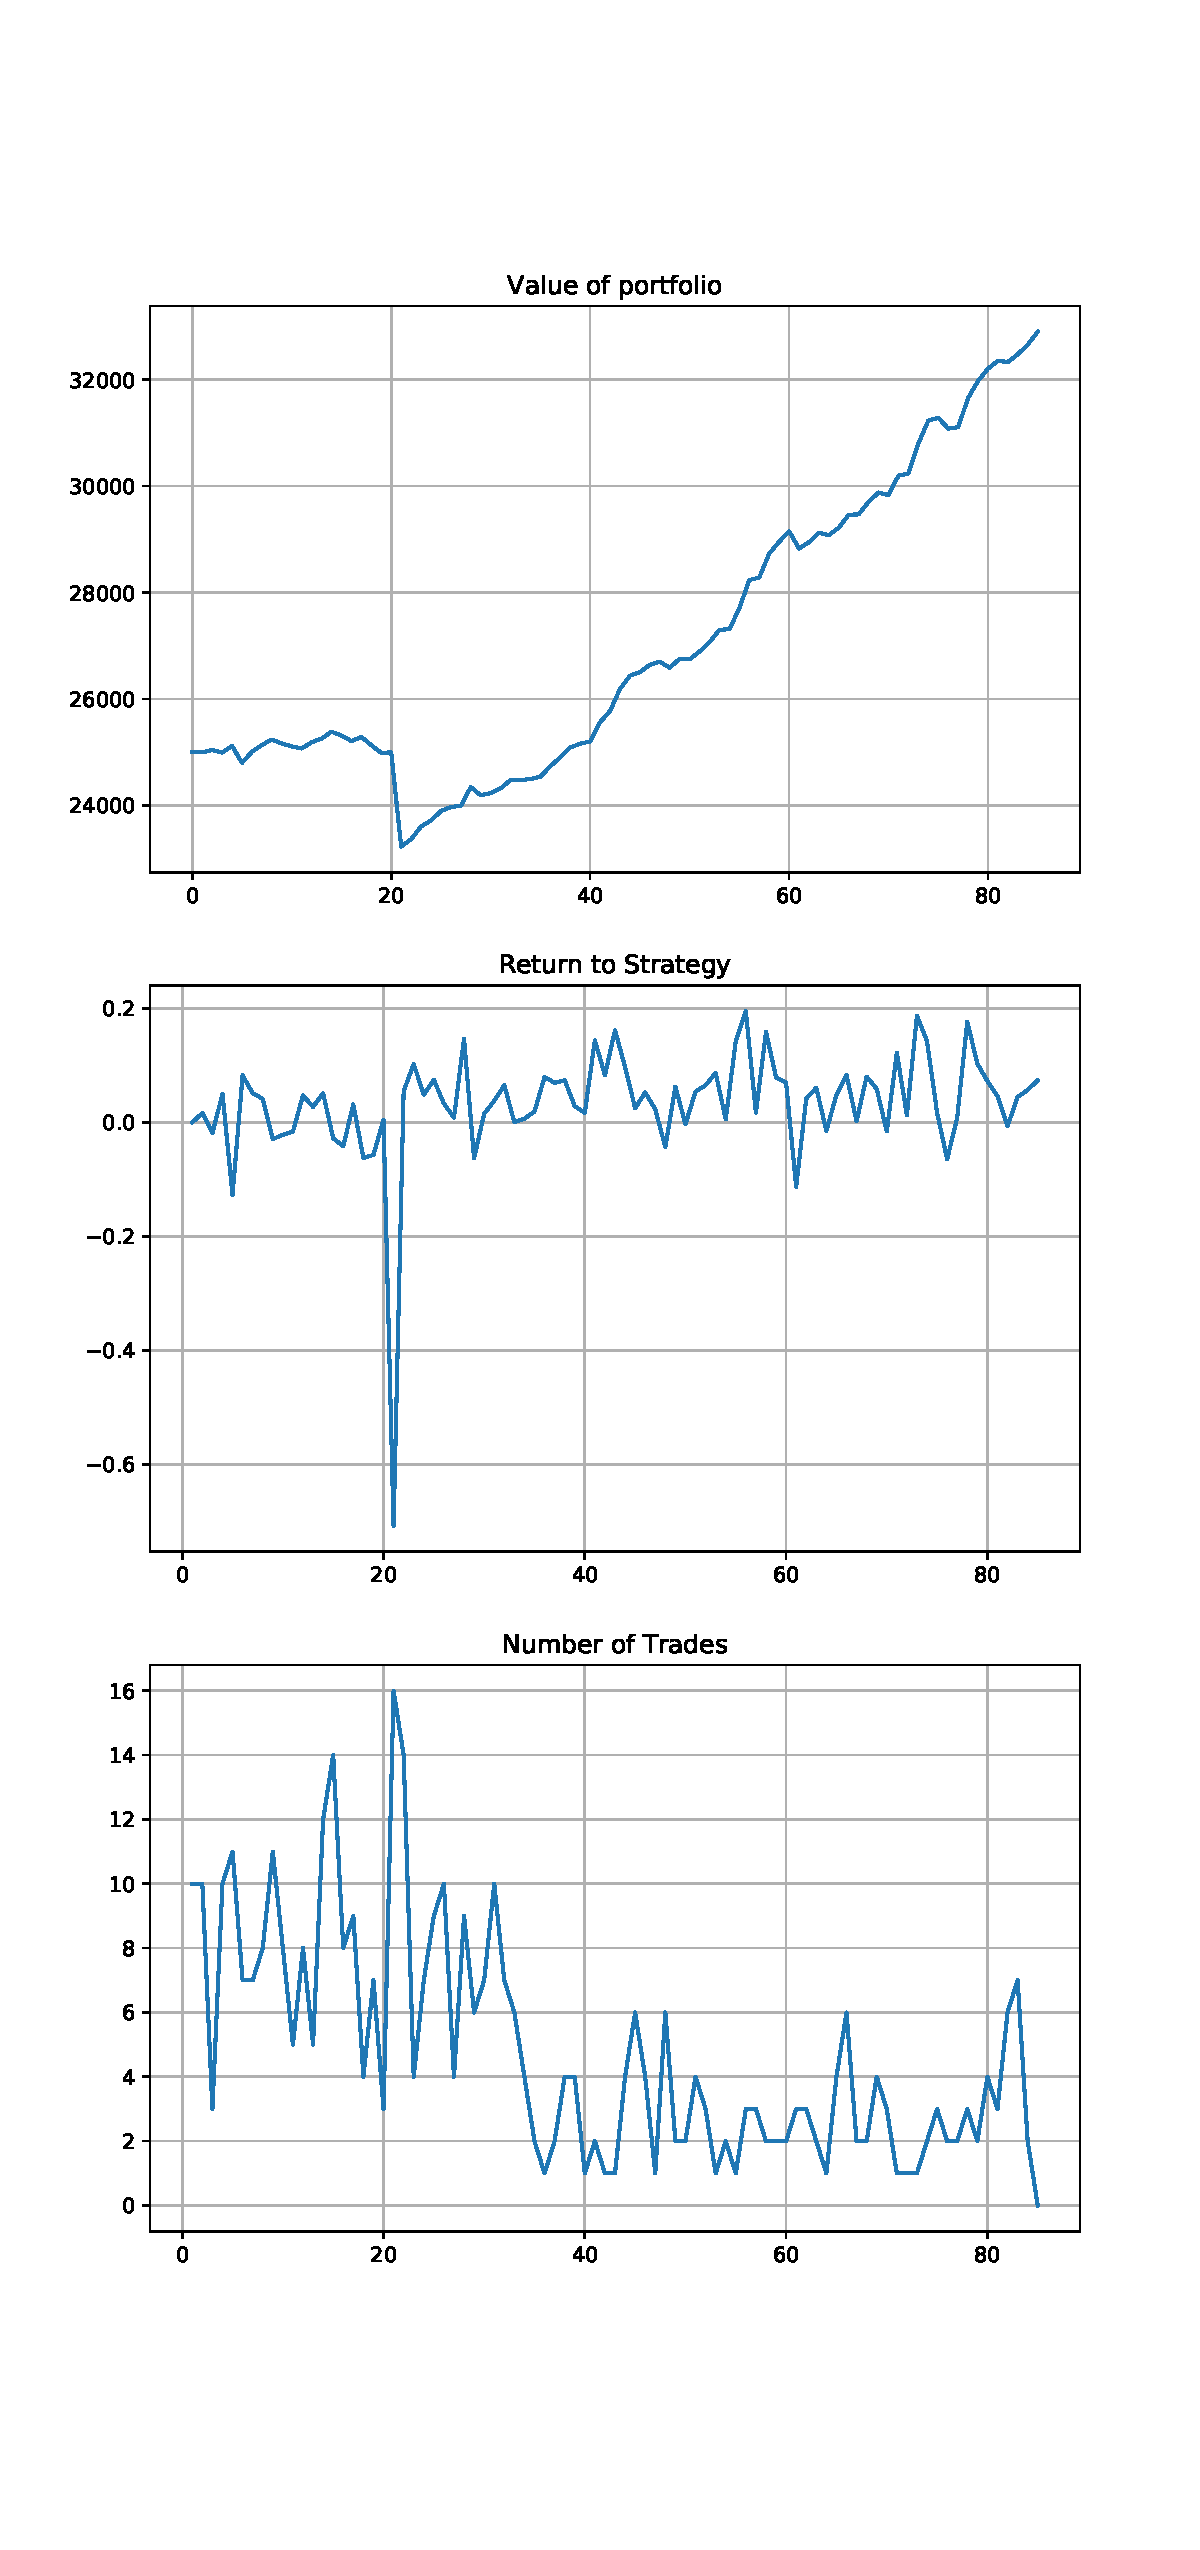
\includegraphics[width=0.75\textwidth]{pump_dump_sim_var_1.pdf}
\label{fig_var_1_sim}
\end{figure}

\pagebreak

\subsection{Default Signal, Entry at 20\% after 2/26/2021}

The default signal shows great improvement after February 26th, 2021. The win rate increases to 70\% and the win-loss ration improves to ~9:7 (see table \ref{tab_var_1_after}). Expected returns improve to 5\%. 

Figures \ref{tab_var_1_after} and \ref{fig_var_1_sim_after} show corresponding results for extended holds and the simulation. The extended holds perform much better, with expected increasing to 10\% on the 5th day of holding, and only 25\% trades ever nearing negative returns. 

\begin{table}
\caption{Performance of Default Signal, Entry at 20\%, After 2/26/2021}
\center{Winners}
\\[2ex]
\begin{tabular}{lcccc}
\hline
         &   0.25   &   0.75   &  median  & average   \\
\midrule
\midrule
constant & 0.0374   & 0.1232   & 0.0727   & 0.0928    \\
         & (0.0077) & (0.0118) & (0.0086) & (0.0073)  \\
N        & 91       & 91       & 91       & 91        \\
Win rate & 0.75     & 0.75     & 0.75     & 0.75      \\
\hline
\end{tabular}

\center{Losers}
\\[2ex]
\begin{tabular}{lcccc}
\hline
          &   0.25   &   0.75   &  median  & average   \\
\midrule
\midrule
constant  & 0.0154   & 0.1010   & 0.0373   & 0.0698    \\
          & (0.0160) & (0.0252) & (0.0178) & (0.0142)  \\
N         & 30       & 30       & 30       & 30        \\
Loss rate & 0.25     & 0.25     & 0.25     & 0.25      \\
\hline
\end{tabular}
\label{tab_var_1_after}
\end{table}

\begin{figure}
\center{Default Signal, 20\% Entry, After 2/26/2021: Average and Quantile Returns By Day Held}
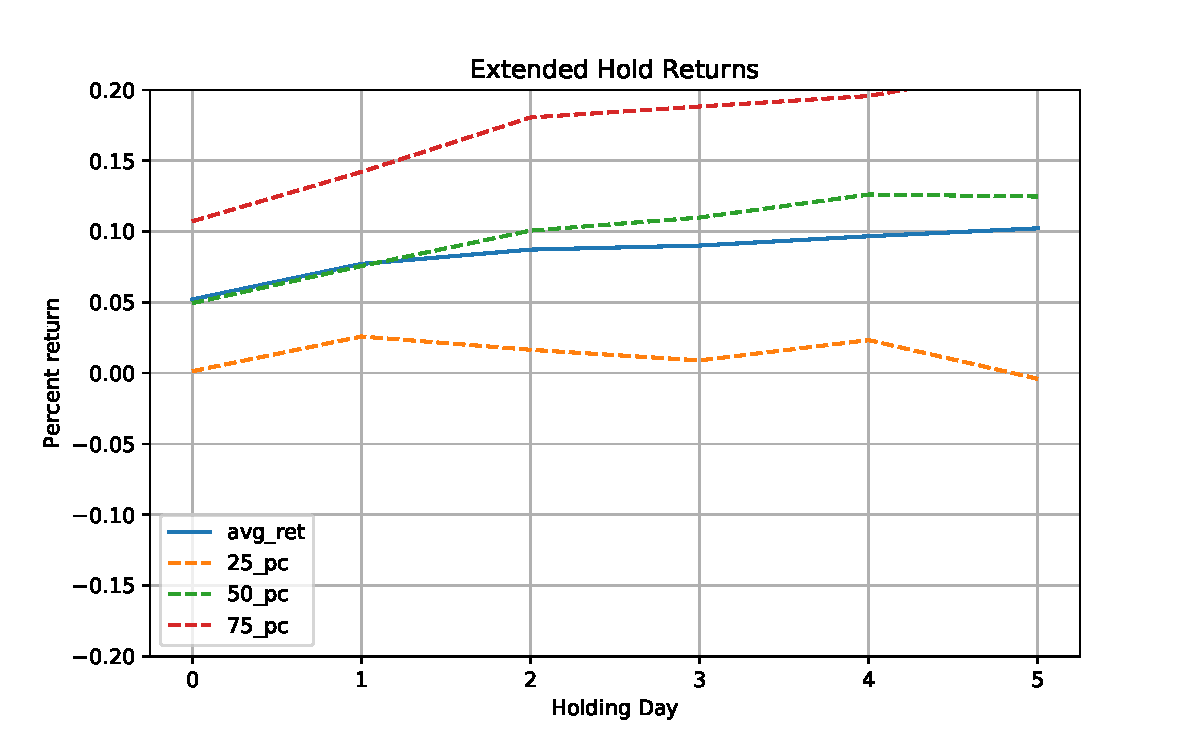
\includegraphics[width=\textwidth]{pump_dump_ext_hold_var_1_after.pdf}
\caption{Extended hold returns are shown. Returns on a holding day are the return if the position was exited on the holding day in question. For example, returns on holding day 0 are returns in stocks were sold at the day the position was entered; returns on day 1, for stocks sold after holding for one day. The quantile returns represent the fraction of stocks with returns worse than the dashed line. for example, the red dashed line shows that 75\% of stocks had returns worse than ~11\% on day 0, ~14\% on day 1, etc.}
\label{fig_var_1_ext_hold_after}
\end{figure}

\begin{figure}
\caption{Default Signal, 20\% Entry, After 2/26/2021: Simulation}
\center
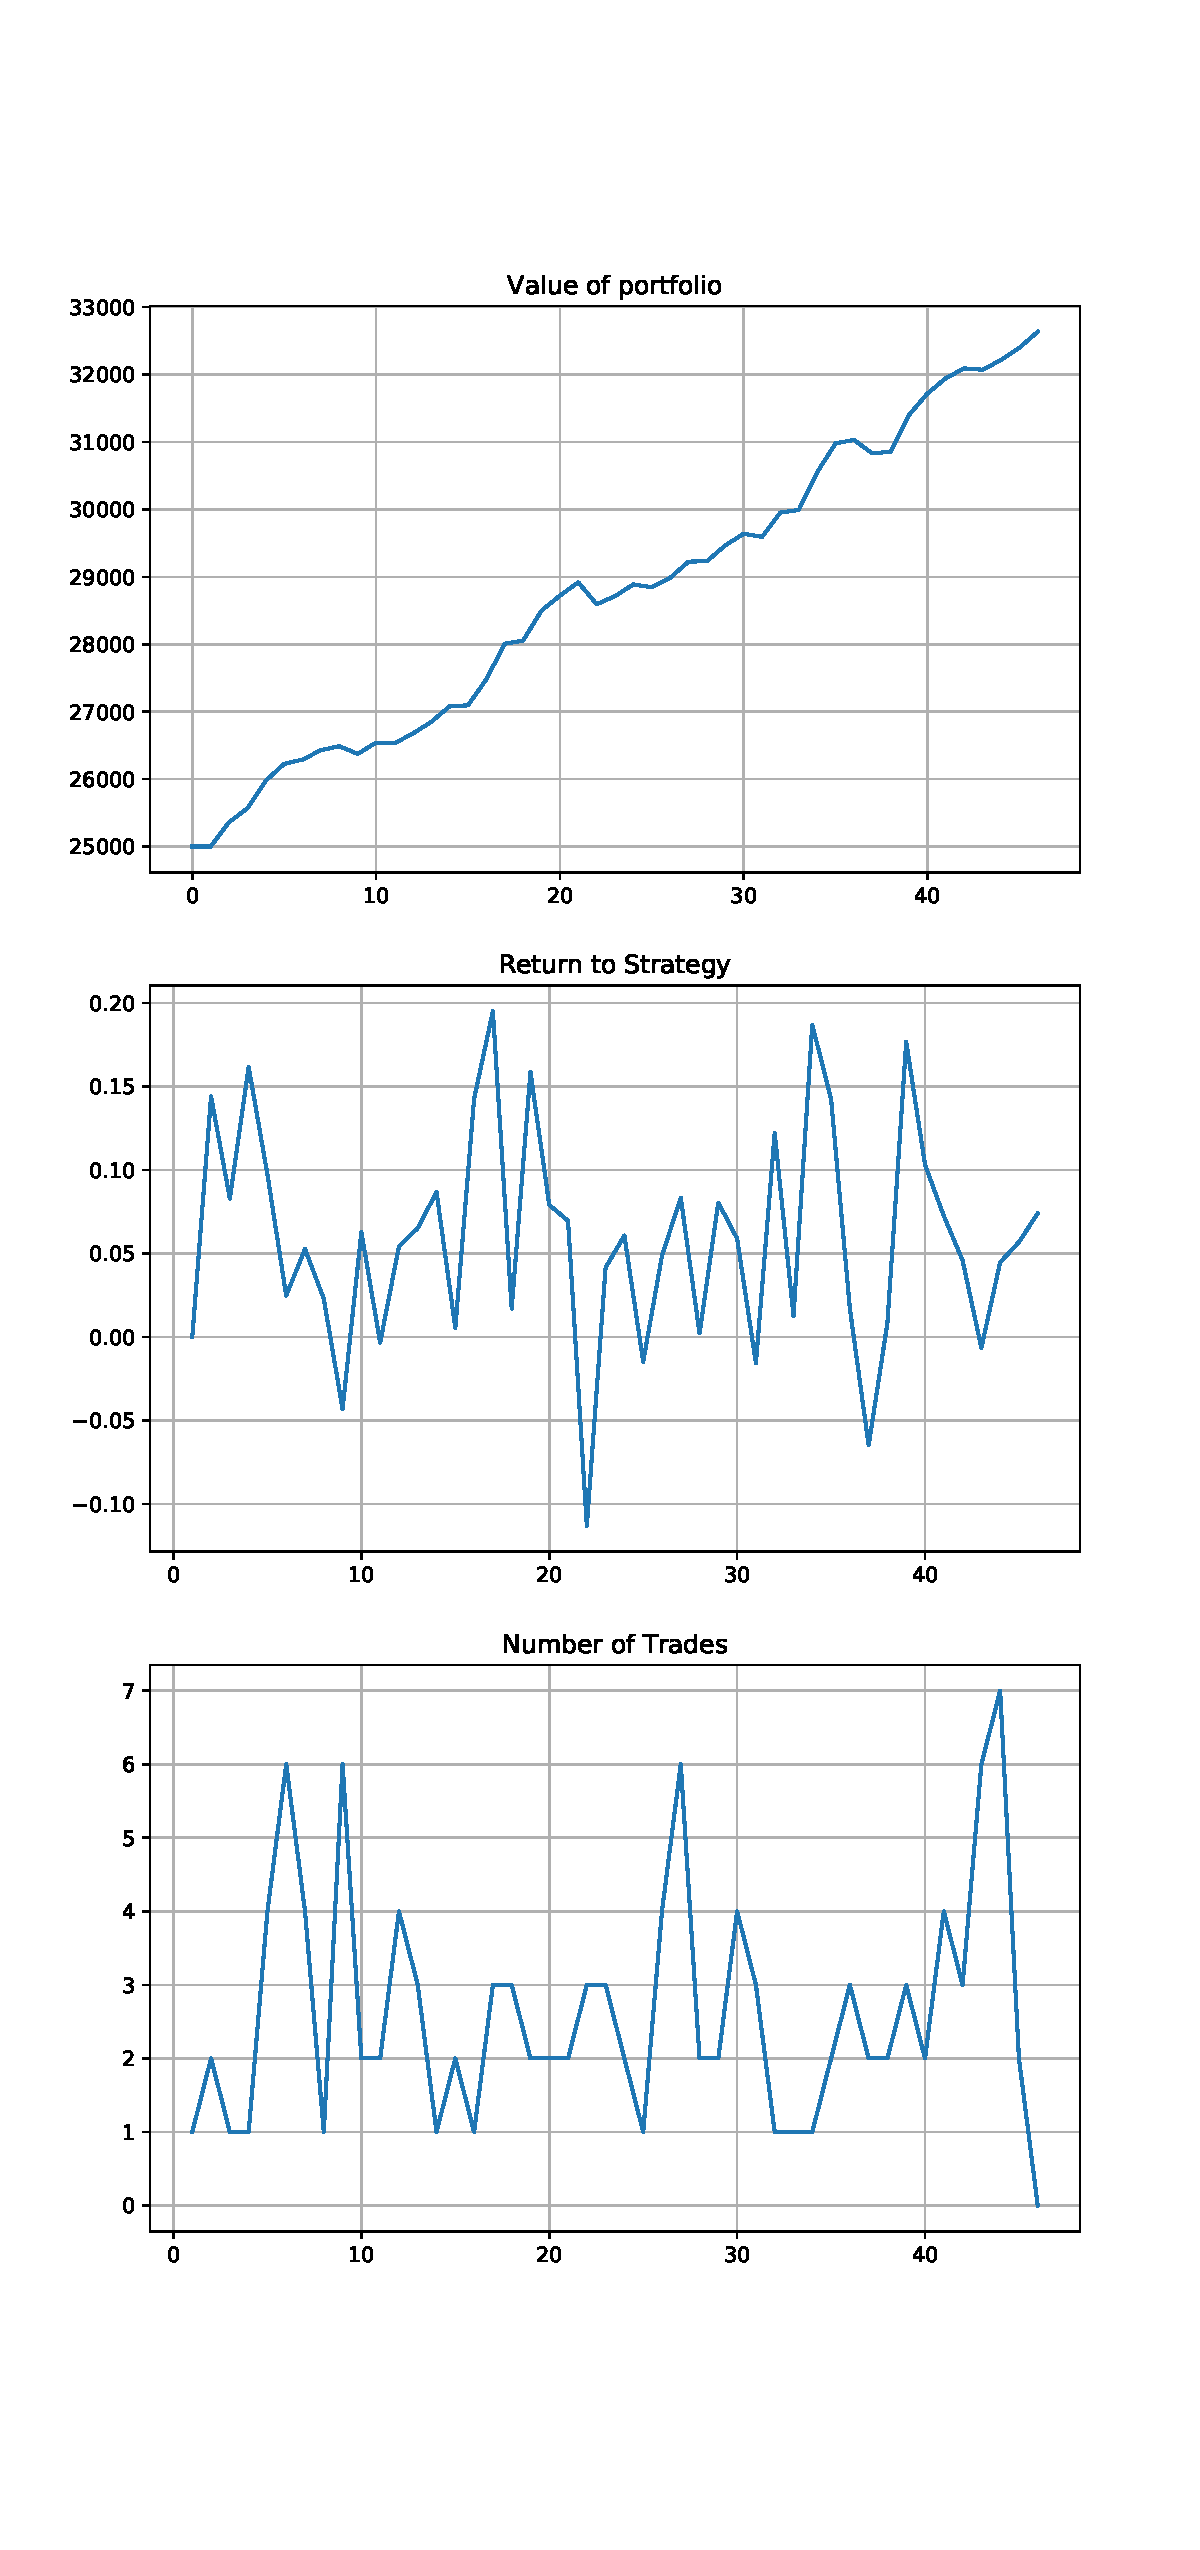
\includegraphics[width=0.75\textwidth]{pump_dump_sim_var_1_after.pdf}
\label{fig_var_1_sim_after}
\end{figure}

\pagebreak

\section{Results: Entry at Average Rise (32\%)}

I then analyzed a variant of the default signal, in which a stock had to rise 32\% from open to be entered into, in addition to closing between \$1 and \$2. 32\% was the average rise of a stock that exhibited the default signal above. 128 trades met this criteria between December 29th, 2020 and May 20th 2021.

This variant performs better than the default. The win rate is 70\% and the win-loss ratio is more extreme at 13:17 (see table \ref{tab_var_2}), but expected returns are 3.5\%. 

\begin{table}
\caption{Performance, Entry at 32\%}
\center{Winners}
\\[2ex]
\begin{tabular}{lcccc}
\hline
         &   0.25   &   0.75   &  median  & average   \\
\midrule
\midrule
constant & 0.0606   & 0.1873   & 0.1136   & 0.1255    \\
         & (0.0109) & (0.0169) & (0.0127) & (0.0096)  \\
N        & 89       & 89       & 89       & 89        \\
Win rate & 0.70     & 0.70     & 0.70     & 0.70      \\
\hline
\end{tabular}

\center{Losers}
\\[2ex]
\begin{tabular}{lcccc}
\hline
          &   0.25   &   0.75   &  median  & average   \\
\midrule
\midrule
constant  & 0.0303   & 0.1563   & 0.0802   & 0.1722    \\
          & (0.0206) & (0.0304) & (0.0222) & (0.0518)  \\
N         & 39       & 39       & 39       & 39        \\
Loss rate & 0.30     & 0.30     & 0.30     & 0.30      \\
\hline
\end{tabular}
\label{tab_var_2}
\end{table}

The extended returns are shown in figure \ref{fig_var_2_ext_hold}. As you can see, the best, worst, and average returns are all improved over the default signal.

I'm skipping the simulation for the whole timer period. I present one for the time frame after 2/26/2021, as I think this is the most relevant.

\begin{figure}
\center{32\% Entry: Average and Quantile Returns By Day Held}
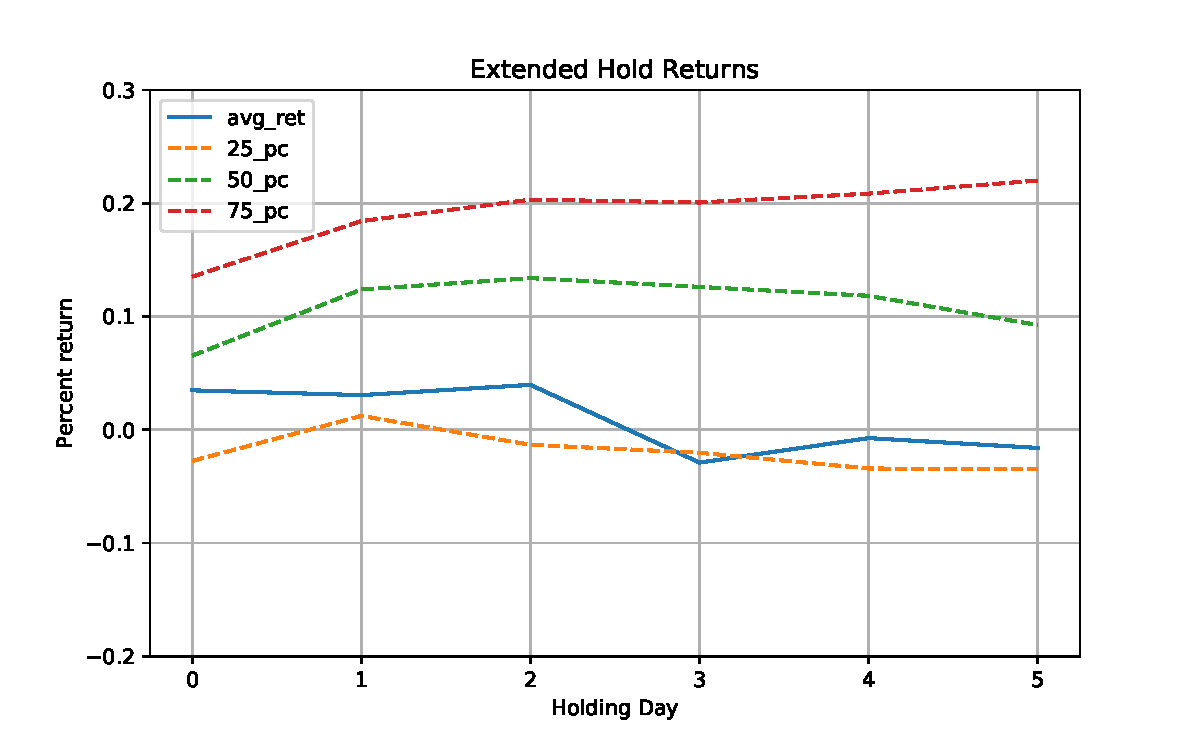
\includegraphics[width=\textwidth]{pump_dump_ext_hold_var_2.pdf}
\caption{Extended hold returns are shown. Returns on a holding day are the return if the position was exited on the holding day in question. For example, returns on holding day 0 are returns in stocks were sold at the day the position was entered; returns on day 1, for stocks sold after holding for one day. The quantile returns represent the fraction of stocks with returns worse than the dashed line. for example, the red dashed line shows that 75\% of stocks had returns worse than ~14\% on day 0, ~19\% on day 1, etc.}
\label{fig_var_2_ext_hold}
\end{figure}

\pagebreak

\subsection{Default Signal, Entry at 20\% after 2/26/2021}

Only 31 trades met this criteria between December 29th, 2020 and May 20th 2021. Still, their great performance may justify the restriction of the signal. 

For an exit on the same day as entry, the win rate is 74\% and the win-loss ration is 2:1 (see table \ref{tab_var_2_after}). Expected returns are 8.8\%. Extended returns are very good. The consistent improvement in returns across quantiles up through the second day of holding might suggest it optimal to hold positions for two days (see figure \ref{fig_var_2_ext_hold_after}).

\begin{table}
\caption{Performance, Entry at 32\%, After 2/26/2021}
\center{Winners}
\\[2ex]
\begin{tabular}{lcccc}
\hline
         &   0.25   &   0.75   &  median  & average   \\
\midrule
\midrule
constant & 0.0313   & 0.1279   & 0.0730   & 0.0956    \\
         & (0.0082) & (0.0127) & (0.0091) & (0.0080)  \\
N        & 101      & 101      & 101      & 101       \\
Win rate & 0.64     & 0.64     & 0.64     & 0.64      \\
\hline
\end{tabular}

\center{Losers}
\\[2ex]
\begin{tabular}{lcccc}
\hline
          &   0.25   &   0.75   &  median  & average   \\
\midrule
\midrule
constant  & 0.0190   & 0.0511   & 0.0303   & 0.0551    \\
          & (0.0080) & (0.0102) & (0.0083) & (0.0156)  \\
N         & 25       & 25       & 25       & 25        \\
Loss rate & 0.35     & 0.35     & 0.35     & 0.35      \\
\hline
\end{tabular}
\label{tab_var_2_after}
\end{table}

\begin{figure}
\center{32\% Entry, After 2/26/2021: Average and Quantile Returns By Day Held}
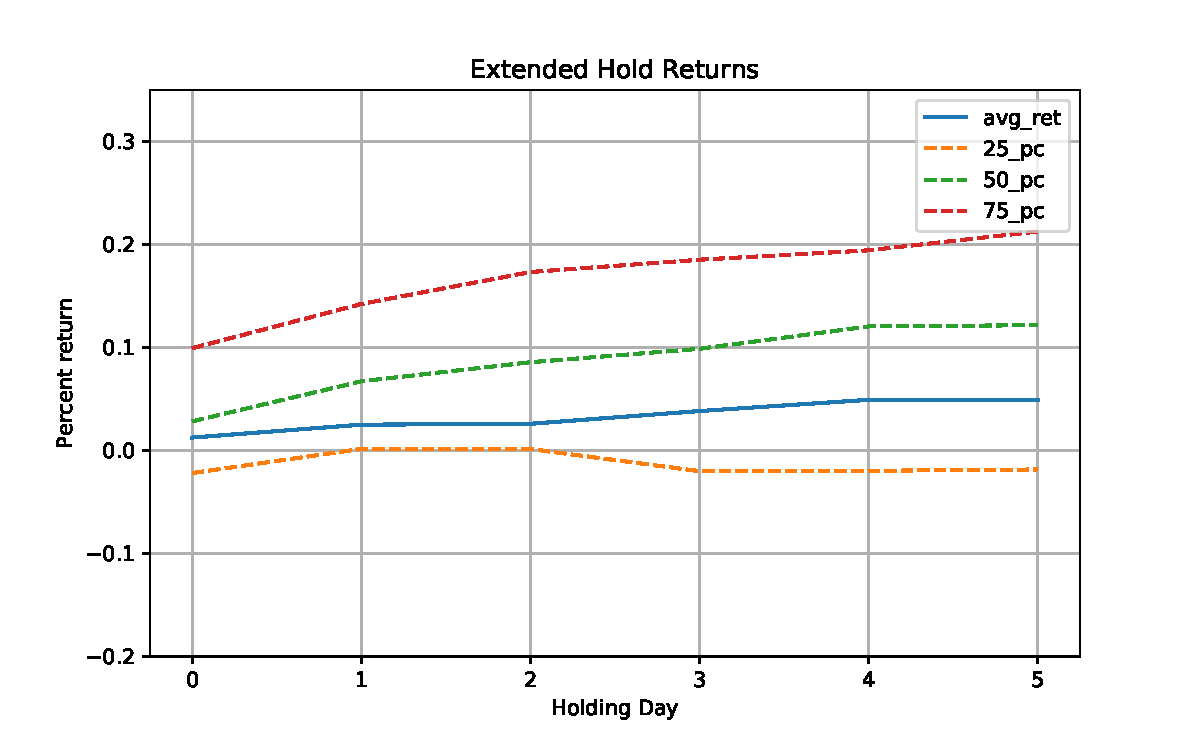
\includegraphics[width=\textwidth]{pump_dump_ext_hold_var_2_after.pdf}
\caption{Extended hold returns are shown. Returns on a holding day are the return if the position was exited on the holding day in question. For example, returns on holding day 0 are returns in stocks were sold at the day the position was entered; returns on day 1, for stocks sold after holding for one day. The quantile returns represent the fraction of stocks with returns worse than the dashed line. for example, the red dashed line shows that 75\% of stocks had returns worse than ~19\% on day 0, ~22\% on day 1, etc.}
\label{fig_var_2_ext_hold_after}
\end{figure}

The simulation results are also good, showing consistent returns (see figure \ref{fig_var_2_sim_after}).

\begin{figure}
\caption{32\% Entry, After 2/26/2021: Simulation}
\center
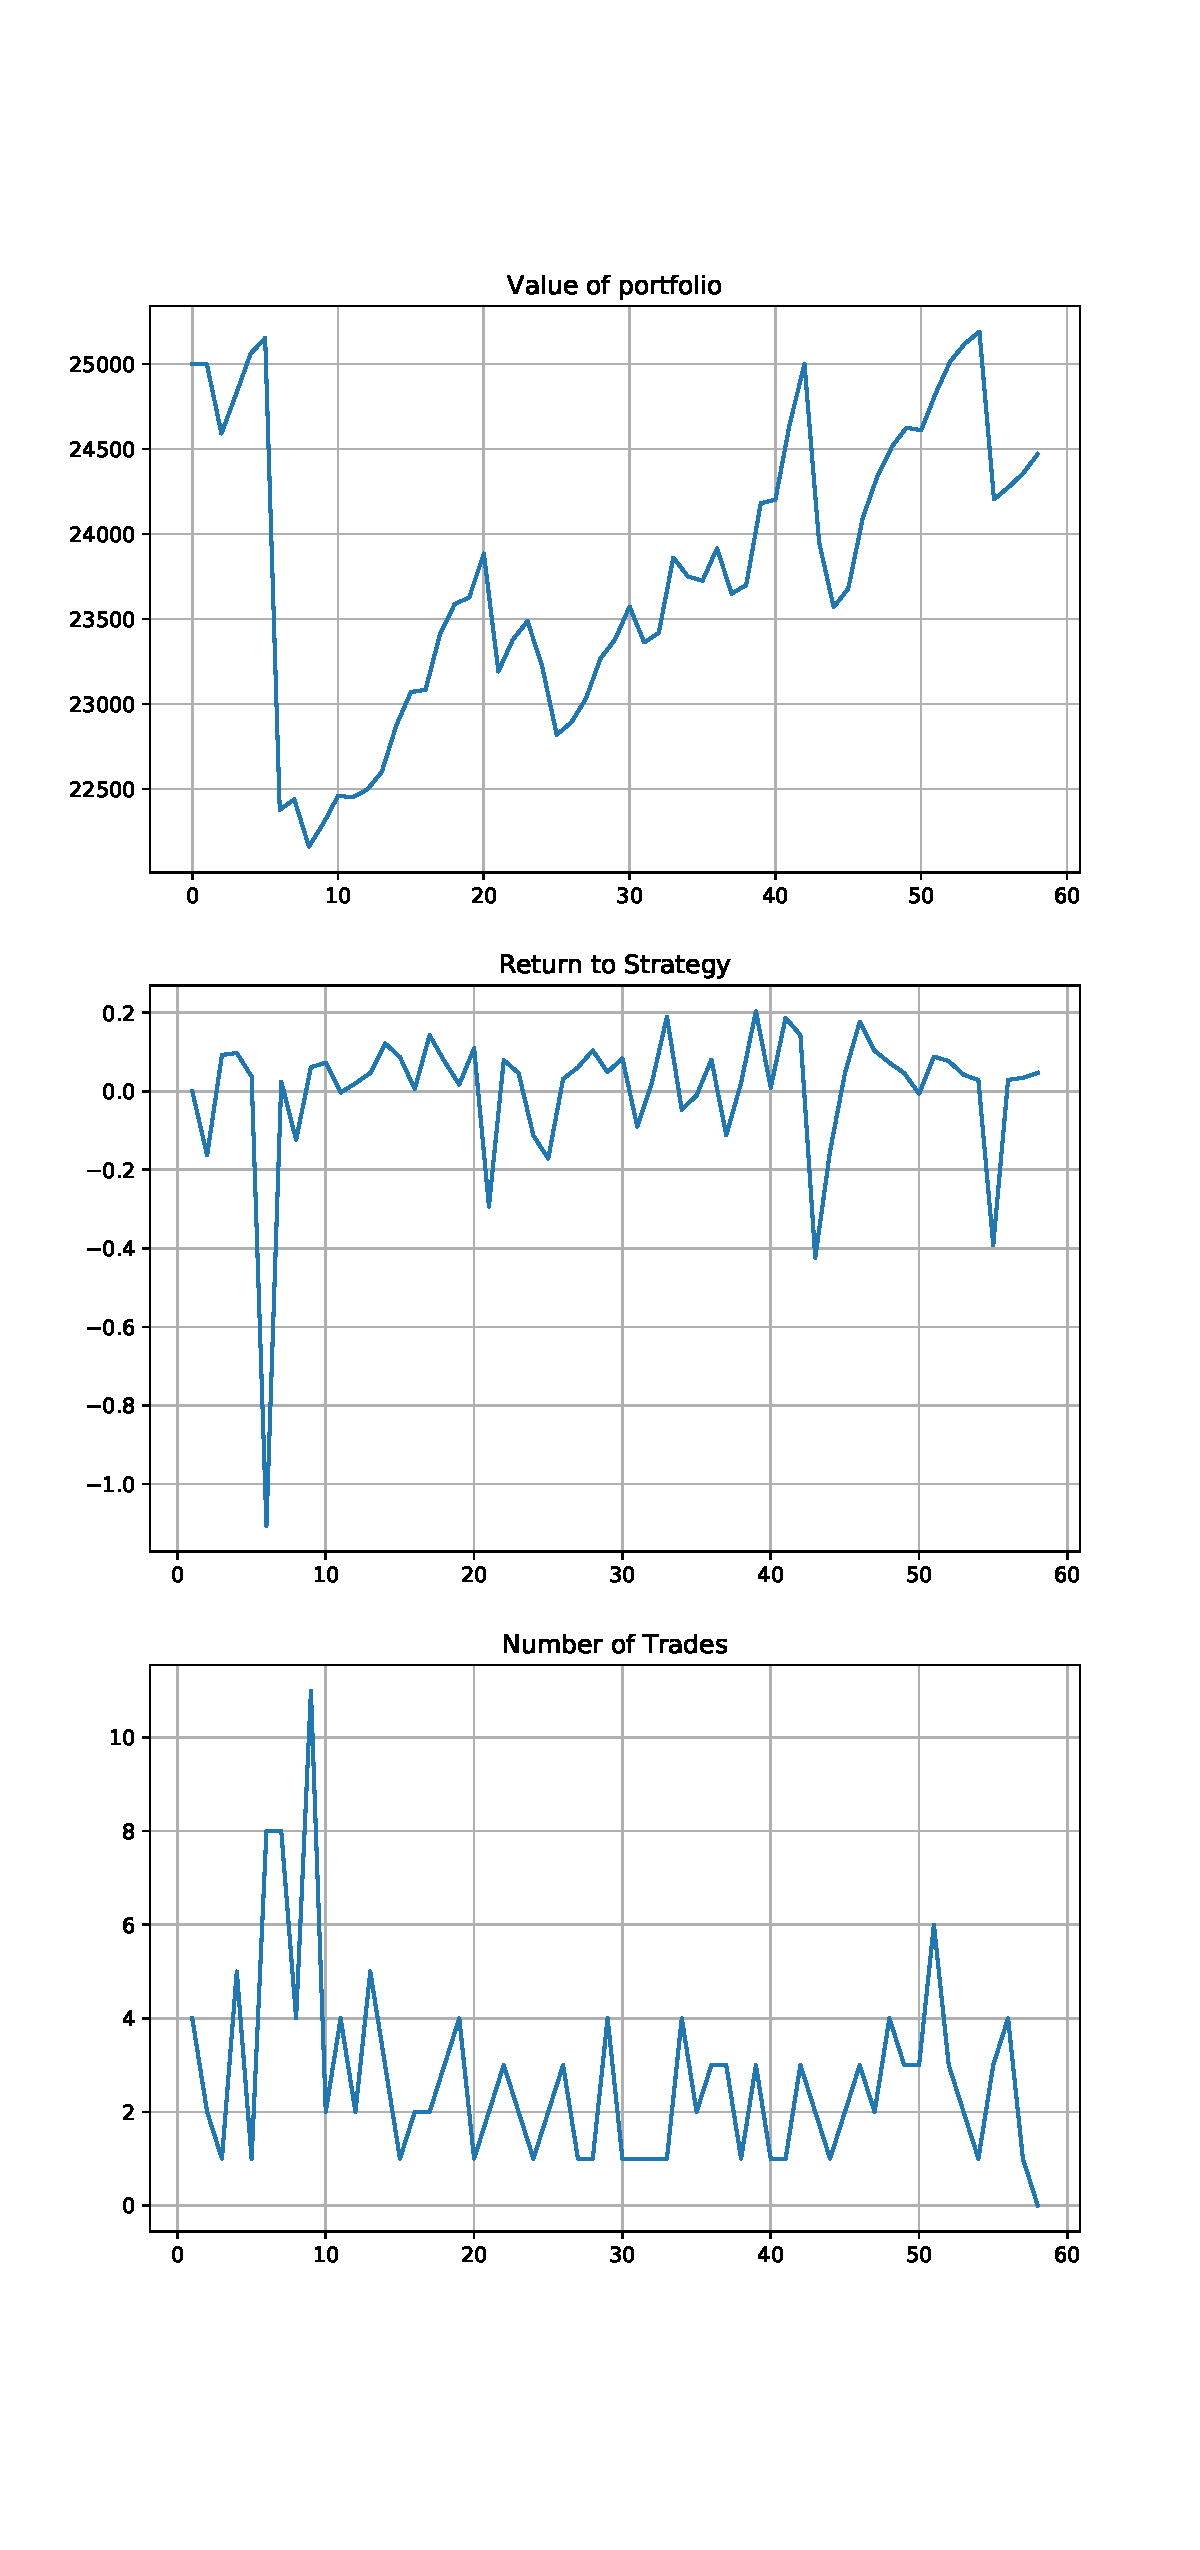
\includegraphics[width=0.75\textwidth]{pump_dump_sim_var_2_after.pdf}
\label{fig_var_2_sim_after}
\end{figure}

\end{document}